\documentclass[a4paper, 10pt, french]{article}

\usepackage[utf8]{inputenc}
\usepackage[T1]{fontenc}
\usepackage[frenchb]{babel}
\usepackage{lmodern}
\usepackage[autolanguage]{numprint}
\usepackage{enumitem}
\usepackage{array}
\usepackage{multirow}
\usepackage{collcell}

\usepackage[margin=3cm]{geometry}
\usepackage{multicol}
\usepackage[10pt]{moresize}
\usepackage{pdflscape}

\usepackage{pdfpages}



\usepackage{amsthm}
\usepackage{amsmath}
\usepackage{amssymb}
\usepackage{mathrsfs}
\usepackage{amsopn}
\usepackage{stmaryrd}


\newcommand{\code}[1]{\texttt{#1}}
\newcommand{\foreign}[1]{\emph{#1}}

\newcommand{\affects}{$\leftarrow$}
\newcolumntype{R}{>{\ttfamily}{l}}
\newcolumntype{M}{>{$}{c}<{$}}
\newcolumntype{U}{>{\code{r1,}}{c}}
\newcolumntype{D}{>{\code{r2,}}{c}}
\newcolumntype{O}{>{\code{o}}{c}}
\newcolumntype{E}{>{$r_1$}{c}}
\newcolumntype{A}{>{\affects}{l}}



\title{Rapport de Systèmes Numériques / Digitaux / Digitals}
\author{Marc \bsc{Ducret} \and Florentin \bsc{Guth} \and Martin \bsc{Ruffel} \and Lionel \bsc{Zoubritzky}}

\begin{document}

\maketitle


\section{Structure du système}

\subsection{Architecture du processeur}

On choisit de stocker les mots sur 32 bits (4 octets). En effet, cela permettra d'utiliser des entiers (signés seulement, pour simplifier) de taille importante. On utilise 8 registres (codés sur 2 bits) en plus du \foreign{program counter}. Les adresse sont codées sur 17 bits, ce qui fait une \foreign{RAM} de 128 Ko.

\subsection{Organisation de la \foreign{RAM}}

\begin{table}[h]
 \centering
 \begin{tabular}{|R|c|c|}
  \hline
  Adresse & Nombre de mots & Données \\
  \hline
  0x00000 & $s_w * s_h$ & Contenu affiché à l'écran (caractères) \\
  \hline
  0x10000 & 1 & Indique si il est nécessaire de redessiner l'écran \\
  0x10001 & 1 & Indique si le programme a terminé son exécution \\
  0x10002 & 1 & Largeur de l'écran $s_w$ \\
  0x10003 & 1 & Hauteur de l'écran $s_h$ \\
  0x10004 & 1 & Temps en secondes depuis le 01/01/1970 00h00 \\
  \hline
  0x10005 & ? & \'Etat du clavier \\
  \hline
  0x11000 & ? & Variables du programme \\
  \hline
 \end{tabular}
 \caption{Organisation de la \foreign{RAM}}
\end{table}


\subsection{Opérations implémentées}

On a fait le choix d'une représentation peu factorisée, donc facile à décoder.

Pour obtenir le code hexadécimal d’une instruction, ajouter le code correspondant à l’opération, plus celui correspondant au(x) registre(s) (multiplié par 8 le cas échéant) plus éventuellement celui de la constante (multiplié par 64 le cas échéant)

Les instructions de décalage (\code{lsl} et \code{lsr}) ne prennent en compte que les 5 derniers bits du registre de décalage. Les instructions contenant une adresse fonctionne de même modulo $2^{17}$. \code{ZF} est le drapeau correspondant à un résultat nul, il est levé ou abaissé par l'instruction précédente.

%\begin{landscape}
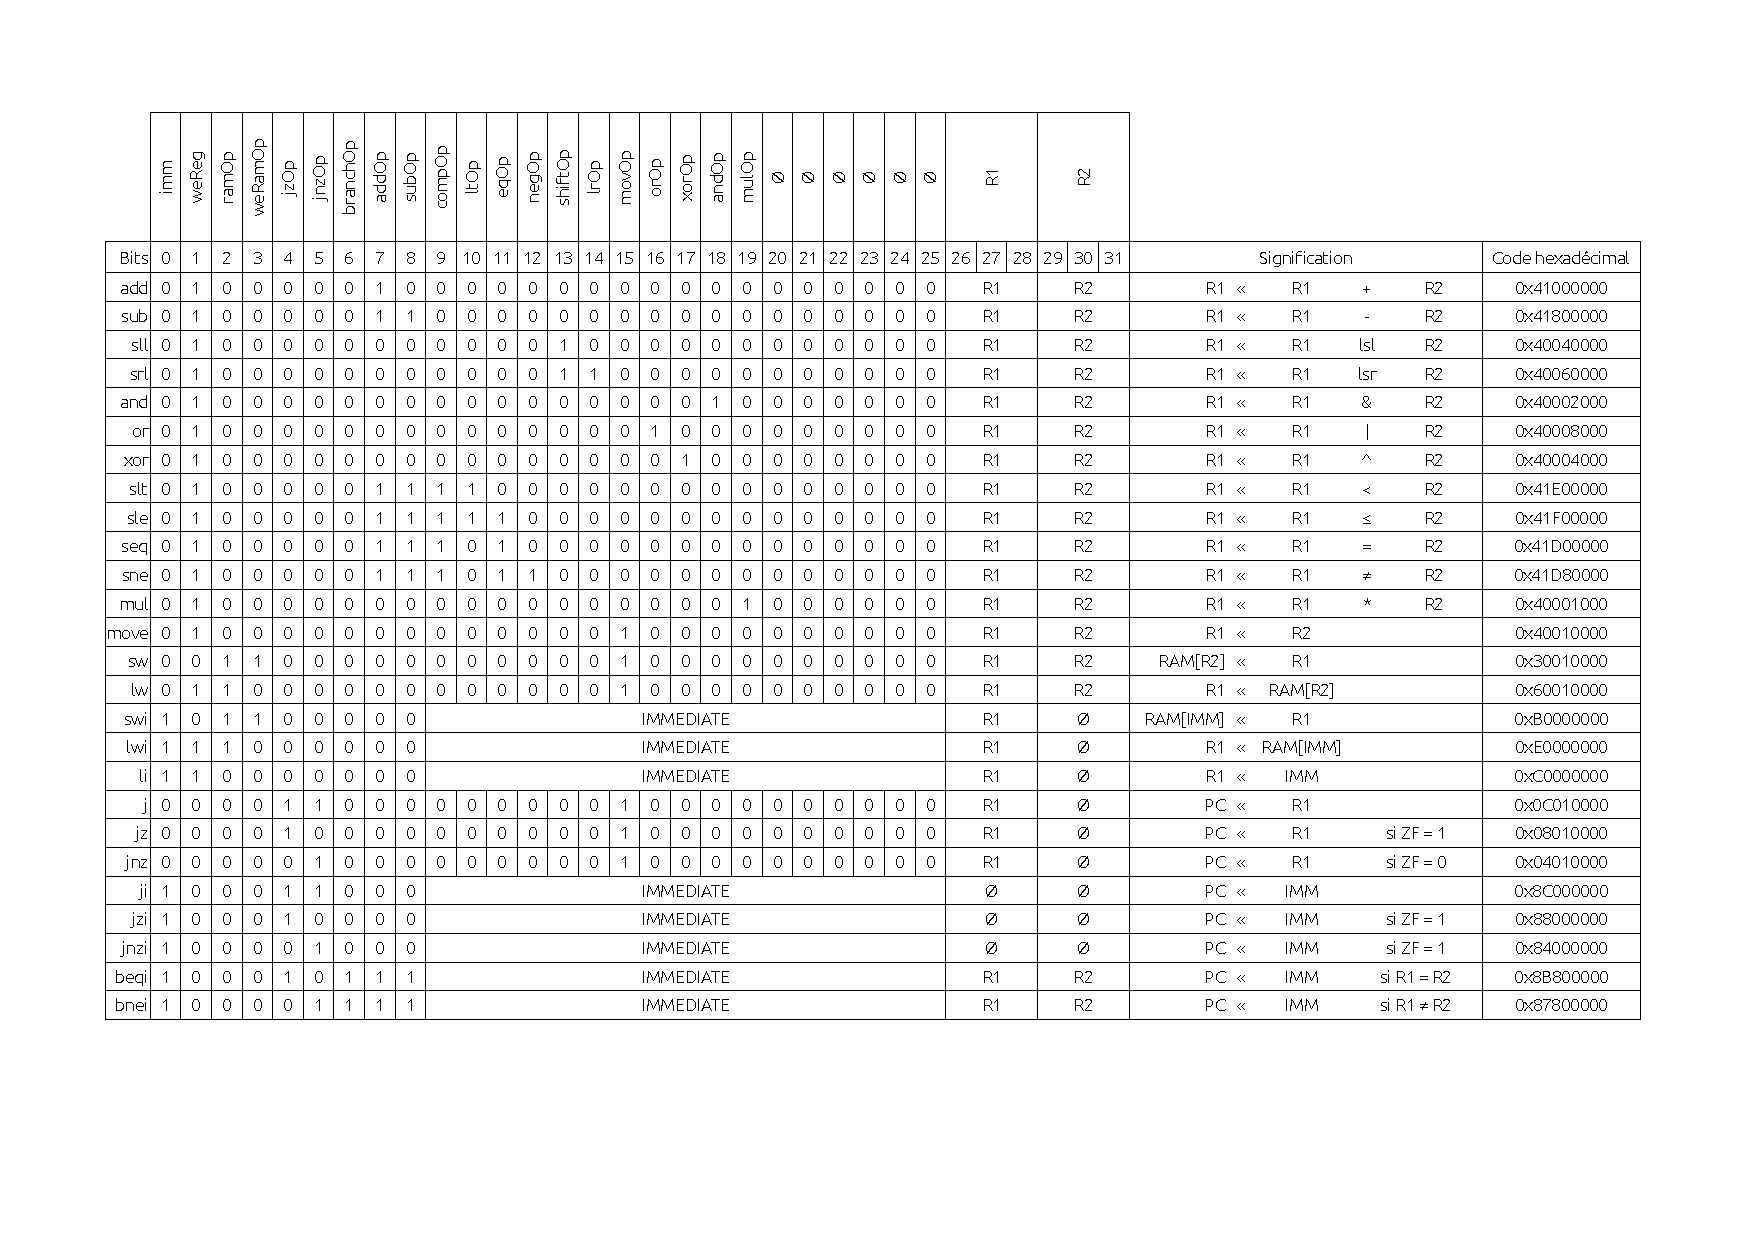
\includepdf[pages={1},landscape=true]{opcodes.pdf}
%\end{landscape}


\section{Processeur}

\subsection{Fonctionnemnt général}

Le processeur est écrit en \foreign{MiniJazz}, puis compilé en \foreign{net-list}. La \foreign{net-list} est ensuite compilée en \foreign{C}, puis en assembleur \code{x86-64} par \foreign{gcc} afin d'être exécutée le plus rapidement possible.

Le code \foreign{MiniJazz} du processeur a été optimisé de la façon suivante :
\begin{itemize}
 \item dérécursification des fonctions pour opérer directement sur 32 bits,
 \item remplacement des nappes de fils par 32 variables,
\end{itemize} dans le but d'éviter au maximum les recopies lors de la simulation du processeur.

\subsection{Architecture du programme \foreign{MiniJazz}}




\section{Montre digitale}

\subsection{Le langage \foreign{Tong}}

On utilise un langage intermédiaire qui sera ensuite compilé en assembleur (de notre processeur) puis en binaire. Ce langage, \foreign{Tong}, dispose des fonctionnalités suivantes :
\begin{itemize}
 \item on peut déclarer des variables globales (représentant des entiers) dans le champ \code{.vars},
 \item on écrit les instructions dans le champ \code{.prgm},
 \item on peut déclarer des fonctions avec la syntaxe \code{@ main}, que l'on appelle avec \code{> main;},
 \item on peut affecter des expressions aux variables : \code{x = (y * 2) \& (5 | a);},
 \item on peut effectuer des tests avec \code{? x = 1 \{ then \} \{ else \}},
 \item on peut effectuer des boucles avec \code{! x < 60 \{ x = x + 1; \}},
 \item on peut effectuer des appels systèmes \code{> draw addr 'c'},
 \item le temps en secondes depuis le 1\ier\ janvier 1970 à minuit est stocké dans la variable \code{time}.
\end{itemize}

\subsection{Compilation du \foreign{Tong}}

Les variables locales reçoivent à la compilation une adresse statique dans la \foreign{RAM}. Les expressions sont quant à elles calculées dans les registres (si le nombre de registres ne suffit pas à calculer l'expression considérée, c'est à l'utilisateur de la découper en deux).

On a choisi de ne pas implémenter de pile. Ainsi, les appels de fonction sont \foreign{inlinés} (on interdit ainsi les fonctions récursives, qui peuvent être réalisées avec une boucle \code{!}), ce qui évite d'avoir à gérer les adresses de retour et privilégie la vitesse plutôt que la taille de l'exécutable.

\end{document}
